\documentclass[a4paper]{ctexart}

\usepackage{fancyhdr}
\usepackage{listings}
\usepackage{xcolor}
\usepackage{amsmath}
\usepackage{algorithm}
\usepackage{graphicx}
\usepackage[noend]{algpseudocode}
\usepackage{physics}
\usepackage{multirow}

% Codes settings
\lstset{
	language=Python,
	numbers = left,
	numberstyle = \tiny,
	basicstyle = \small,
	keywordstyle = \color{blue!70}\bfseries,
	stringstyle = \color{red},
	commentstyle =\color[rgb]{0.6,.6,.6}\itshape,
	identifierstyle={},
	frame = shadowbox,
	rulesepcolor= \color{ red!20!green!20!blue!20},
	escapeinside=``
}

%Page setting
\pagestyle{fancy}
\rfoot{\thepage}
\cfoot{}
\lfoot{\itshape Jeffreyyao@pku.edu.cn}
\setlength{\abovecaptionskip}{0.05cm}
\setlength{\belowcaptionskip}{0.05cm}

\title{计算物理第三次开卷考试}
\author{姚铭星 1700011321}
\date{}

\begin{document}
\maketitle
\section{第一题:原子的激发谱}
\subsection{基态的求解}
对于数值求解不含时薛定谔方程:
\begin{equation}
\left[-\frac{1}{2} \frac{d^{2}}{d x^{2}}+V(x)\right] \psi(x)=E_{n} \psi(x)
\end{equation}
可以将二阶导数该为有限差分
\begin{equation}
\partial_{x}^{2} \psi\left(x_{i}\right)=\frac{\psi\left(x_{i+1}\right)-2 \psi\left(x_{i}\right)+\psi\left(x_{i-1}\right)}{(\Delta x)^{2}}+o\left((\Delta x)^{2}\right)
\end{equation}
这样可以将哈密顿量表示为三对角对称矩阵的形式:
\begin{equation}
\left(H_{0}\right)_{i j}=\left\{\begin{array}{ll}{\frac{1}{(\Delta x)^{2}}-\frac{1}{\sqrt{x_{i}^{2}+2}},} & {i=j} \\ {\frac{-1}{2(\Delta x)^{2}},} & {|i-j|=1} \\ {0,} & {|i-j|>1}\end{array}\right.
\end{equation}
注意,此处已经使用了边界条件:
\begin{equation}
\psi(x_{-1})=\psi(x_{N})=0
\end{equation}
这样问题变为求解本征值问题:
\begin{equation}
H_0\psi = E_0 \psi
\end{equation}
由于已经给定近似的能量值$E_0=-0.48$,利用原点位移的方法可以直接将问题转化为求解差值的问题。这样可以保证反幂法的顺利运行。

定义新的矩阵$A$为:
\begin{equation}
A = H_0 + 0.48I
\end{equation}
此时利用Cholesky分解(在第一次作业中已经实现过)实现类似于求逆的操作

\subsection{时间演化}
对于加上电场之后的含时的薛定谔方程,与上问中的哈密顿量只差相差一个对角阵:
\begin{equation}
\mathcal{H}(t)=\mathcal{H}_{0}+x E(t)
\end{equation}
因此此时哈密顿量仍然保有三对角形式,并且为实对称矩阵。在时空上划定格点将方程离散化后得到:

\begin{equation}
\begin{aligned}
\psi_{i}^{(j)}&=\psi\left(x_{i}, t_{j}\right)\\
i\frac{\psi_{i}^{(j+1)}-\psi_{i}^{(j)}}{\Delta t}&=\mathcal{H}(t)\psi(t)
\end{aligned}
\end{equation}

为了保证体系的守恒量不受破坏,我们采用辛算法Crank-Nicolson(欧拉中点算法),其格式为:
\begin{equation}
\mathrm{i} \frac{\psi_{i}^{(j+1)}-\psi_{i}^{(j)}}{\Delta t}=\sum_{l} H\left(t_{j+1 / 2}\right)_{i l} \psi_{l}\left(t_{j+1 / 2}\right)=\sum_{l} \frac{1}{2} H\left(t_{j+1 / 2}\right)_{i l}\left(\psi_{l}^{(j)}+\psi_{l}^{(j+1)}\right)
\end{equation}
这样,每一步递推变成求解线性方程问题:
\begin{equation}
\left(1+\frac{\mathrm{i} \Delta t}{2} H\left(t_{j+1 / 2}\right)\right) \psi^{(j+1)}=\left(1-\frac{\mathrm{i} \Delta t}{2} H\left(t_{j+1 / 2}\right)\right) \psi^{(j)}
\end{equation}
而不难发现,此时的Crank-Nicolson形式有幺正性质,即满足:
\begin{equation}
U_jU^{\dagger}_j=1
\end{equation}
因此只需在最初的波函数满足归一化条件,之后的波函数归一化条件自动满足,这样可以直接计算重叠积分:\begin{equation}
P_{0}(t)=\left|\left\langle\psi_{0}(x) | \psi(x, t)\right\rangle\right|^{2}
\end{equation}
\subsubsection{代码实现}
\begin{lstlisting}
def Time_evolution(psi0,xmax,N,dt = .05,T_max = 18*2*np.pi):
	'''
	第一题第二问含时演化问题
	'''
	Dx = 2*xmax/(N-1)
	Nt = int(T_max/dt)
	E0 = np.sqrt(10**(16-16)/3.5094448314)
	H0 = [[1/Dx**2-1/np.sqrt((i)**2+2) for i in\
	np.linspace(-xmax,xmax, N)], [-1/(2*Dx**2) for i in\
	range(N-1)]]  # t=0时哈密顿量
	psi = deepcopy(psi0)
	sequence =[]
	sequence.append(1)
	for t in np.linspace(0,T_max,Nt):
		print("t = "+str(t))
		t1 = t+ .5*dt
		dH = [x*E0*np.sin(t1/(2*18))**2*np.sin(t1) for x in \	
		np.linspace(-xmax,xmax,N)] # 计算哈密顿量含时项
		H = [[H0[0][i]+dH[i] for i in range(N)],[each for each in H0[1]]]
		b = multi([[1-.5j*dt*each for each in H[0]],
		[-.5j*dt*each for each in H[1]]], psi[:])
		L = cholesky([[1+.5*1j*dt*each for each in H[0]],
		[.5*1j*dt*each for each in H[1]]])
		v = solve(L,deepcopy(b))
		psi = deepcopy(v)
		res = abs(sum([psi[i]*psi0[i].conjugate() for i in\
		range(N)]))**2
		sequence.append(res)
	return sequence,psi
\end{lstlisting}
在代码实现过程中,矩阵求逆使用的是第一次作业中的Cholesky方法。
\subsection{动量谱}
将末态波函数去除掉基态重叠的部分,直接进行离散傅里叶变换就可以求得动量谱
\begin{equation}
P(k)=\left|\left\langle\psi_{k} | \psi_{f}\right\rangle\right|^{2}
\end{equation}
\subsection{谐波功率谱}
通过计算偶极矩和加速度两种方法可以计算辐射谐波的功率谱$A(\omega)$
\begin{equation}
\begin{aligned} d(t) &=\langle\psi(t)|x| \psi(t)\rangle \\ A(\omega) &=\frac{-\omega^{2}}{\sqrt{2 \pi}} \int_{0}^{t_{f}} \mathrm{d} t \mathrm{e}^{-\mathrm{i} \omega t} d(t) \\ a(t) &=\left\langle\psi(t)\left|-\partial_{x} V+E(t)\right| \psi(t)\right\rangle \\ A(\omega) &=\frac{1}{\sqrt{2 \pi}} \int_{0}^{t_{f}} \mathrm{d} t \mathrm{e}^{-\mathrm{i} \omega t} a(t) \end{aligned}
\end{equation}

\section{第二题:氢离子电离的动力学模拟}
在强场激光下,原子有一定几率通过隧穿电离成为自由电子,经过经典运动可以运动到无穷远处。本问题考察的是在无穷远处的动量分布。
\subsection{初态制备}
在经典动力学模拟之前,电子需要先经过电离过程,题目中通过蒙卡方法对初态电子分布进行采样:
\begin{equation}
W\left(t, v_{\perp}\right)=\frac{C}{(E(t))^{2}} \exp \left(\frac{-2}{3 E(t)}-\frac{v_{\perp}^{2}}{E(t)}\right)
\end{equation}
采样可以看成是一个速度的高斯分布和一个权重因子的乘积

关于高斯分布,采用第二类舍选法进行采样,采样的效率为:
\begin{equation}
L=\frac{1}{\sqrt{\pi E}} \exp \left(\frac{E}{4}\right)
\end{equation}
\subsubsection{具体实现}
\begin{lstlisting}
class sample:
	'''
	取样类
	'''
	omega = 0
	A0 = 0
	def __init__(self,t,o=0.057,A0=1.325):
		self.omega = o
		self.A0 = A0
		self.t = t
		self.F = Field(o,A0)
		self.E_t=np.sqrt(sum([each**2 for each in self.F.E(t)]))
	
	def gaussian(self):
		'''
		采用第二类舍选法采样一次
		输出采样电子速度v_h的模值
		'''
		repeat = True
		while repeat:
			s1 = random.uniform(0,1)
			s2 = random.uniform(0,1)
			x = - np.log(s1)
		if (x - self.E_t/2)**2<-self.E_t*np.log(s2):
			return x
\end{lstlisting}
\subsubsection{高斯分布}
\subsection{库伦作用下的电子运动}
当每个时刻抽出一个电子之后,它将按哈密顿方程运动
\begin{equation}
\begin{aligned} \frac{\mathrm{d} \mathbf{r}}{\mathrm{d} t} &=\mathbf{p} \\ \frac{\mathrm{d} \mathbf{p}}{\mathrm{d} t} &=-\nabla V(\mathbf{r})-\mathbf{E}(t)=\frac{-\mathbf{r}}{\sqrt{\mathbf{r}^{2}+0.2^{2}}}-\mathbf{E}(t) \end{aligned}
\end{equation}
运动直到$t_{final}=4\pi/\omega$,其中电场强度可以解析算出
\begin{equation}
\mathbf{E}_{l}=\omega A_{0}\left(\frac{1}{8} \sin \frac{\tau}{4} \sin \tau-\cos ^{2} \frac{\tau}{8} \cos \tau\right)\left.\mathbf{e}_{x}\right|_{\tau=\omega t}
\end{equation}
\begin{equation}
\mathbf{E}_{e}=\frac{\omega A_{0}}{\sqrt{1+P^{2}}}\left.\left(\left(\frac{1}{8} \sin \frac{\tau}{4} \sin \tau-\cos ^{2} \frac{\tau}{8} \cos \tau\right) \mathbf{e}_{x}+P\left(\frac{1}{8} \sin \frac{\tau}{4} \cos \tau+\cos ^{2} \frac{\tau}{8} \sin \tau\right) \mathbf{e}_{y}\right)\right|_{\tau=\omega t}
\end{equation}
电子演化使用的是RK-4方法。

当电场停止作用时,体系将只在库伦势下运动,满足一系列守恒关系,从而可以将无穷远处电子动量分布用末态电子状态表示:
\begin{equation}
\begin{aligned} E_{\text { pureCoulomb }} &=\frac{1}{2} p_{f}^{2}-\frac{1}{r_{f}}=\frac{1}{2} p_{\infty}^{2} \\ \mathbf{L} &=\mathbf{r}_{f} \times \mathbf{p}_{f} \\ \mathbf{a} &=\mathbf{p}_{f} \times \mathbf{L}-\frac{\mathbf{r}_{f}}{r_{f}} \end{aligned}
\end{equation}
可以解得
\begin{equation}
\mathbf{p}_{\infty}=p_{\infty} \frac{p_{\infty}(\mathbf{L} \times \mathbf{a})-\mathbf{a}}{1+\left(p_{\infty} L\right)^{2}}
\end{equation}
\subsubsection{代码实现}
\begin{lstlisting}
class electron:
	'''
	电子类
	'''
	q = [0,0]
	def __init__(self,v,t0,type,o=0.057,A0=1.325):
		self.t0 = t0
		self.p = v
		self.F = Field(o,A0,type)
		self.q = [-0.5*self.F.E(t0)[0]/self.F.E_amp(t0)** 2,
		-0.5*self.F.E(t0)[1]/self.F.E_amp(t0)**2]
	
	def __p_evolve(self,q,t):
		return
		[-self.F.E(t)[0]-q[0]/(q[0]**2+q[1]**2+0.2**2)**1.5,
		-self.F.E(t)[1]-q[1]/(q[0]**2+q[1]**2+0.2**2)**1.5]
	
	def __q_evolve(self,p,t):
		return p[:]
	def evolve(self,dt = 0.1,T=2*np.pi/0.057):
		'''
		利用RK4进行牛顿力学模拟
		'''
		n=2
		t_s = np.linspace(self.t0,2*T,int((2*T-self.t0)/dt))
		# x,y = [],[]
		for t in t_s:
			# RK4计算哈密顿方程
			kq1 = self.__q_evolve(self.p,t)
			kp1 = self.__p_evolve(self.q,t)
			kq2 = self.__q_evolve([self.p[i]+.5*dt*kp1[i]\
			 for i in range(n)],t+0.5*dt)
			kp2 = self.__p_evolve([self.q[i]+.5*dt*kq1[i]\
			 for i in range(n)],t+0.5*dt)
			kq3 = self.__q_evolve([self.p[i]+.5*dt*kp2[i]\
			 for i in range(n)],t+0.5*dt)
			kp3 = self.__p_evolve([self.q[i]+.5*dt*kq2[i]\
			 for i in range(n)],t+0.5*dt)
			kq4 = self.__q_evolve([self.p[i]+dt*kp3[i]\
			for i in range(n)],t+dt)
			kp4 = self.__p_evolve([self.q[i]+dt*kq3[i]\ 
			for i in range(n)],t+dt)
			# 更新p,q
			self.p = [self.p[i]+dt/6*(kp1[i]+2*kp2[i]+2*kp3[i]+kp4[i])\
			for i in range(n)]
			self.q = [self.q[i]+dt/6*(kq1[i]+2*kq2[i]+2*kq3[i]+kq4[i])\
			for i in range(n)]
			# x.append(self.q[0])
			# y.append(self.q[1])
		pf = np.sqrt(sum([each**2 for each in self.p]))
		rf = np.sqrt(sum([each**2 for each in self.q]))
		p_inf = np.sqrt(pf**2-2/rf)
		L = self.q[0]*self.p[1]-self.q[1]*self.p[0] # z右手方向为正
		a = [self.p[1]*L-self.q[0]/rf,-self.p[0]*L-self.q[1]/rf]
		return [p_inf*(p_inf*(-L*a[1])-a[0])/(1+p_inf**2*L**2), p_inf*(p_inf*(L*a[0])-a[1])/(1+p_inf**2*L**2)]
\end{lstlisting}
\subsection{结果讨论与展示}
下图是动量谱的模拟结果和线动量分布的统计结果。在采样率约为10000,$dt=0.05$的参数选择下,程序经过一整夜的时间得到了一下结果。
\begin{figure}[hbt]
	\centering
	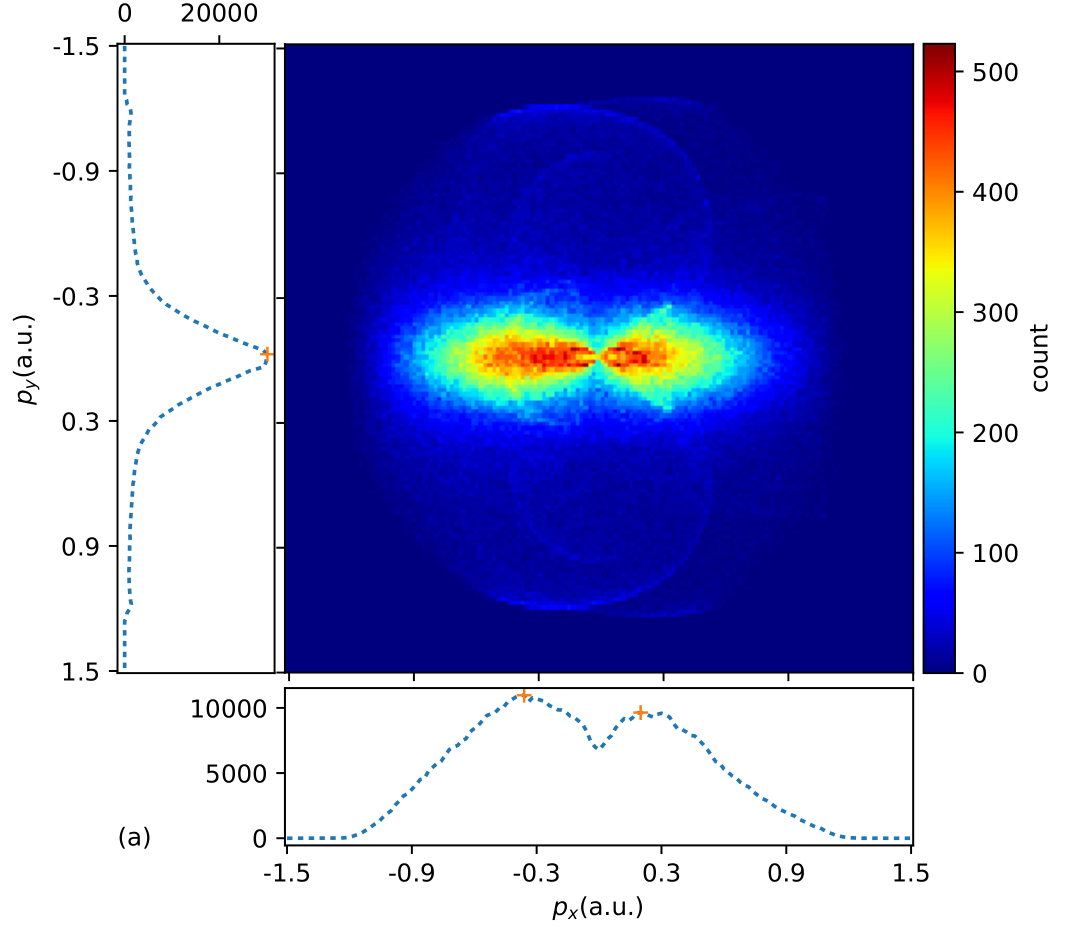
\includegraphics[width=10cm]{./fig/Prob2_3.png}
	\caption{线偏振情况}
\end{figure}
\begin{figure}[hbt]
	\centering
	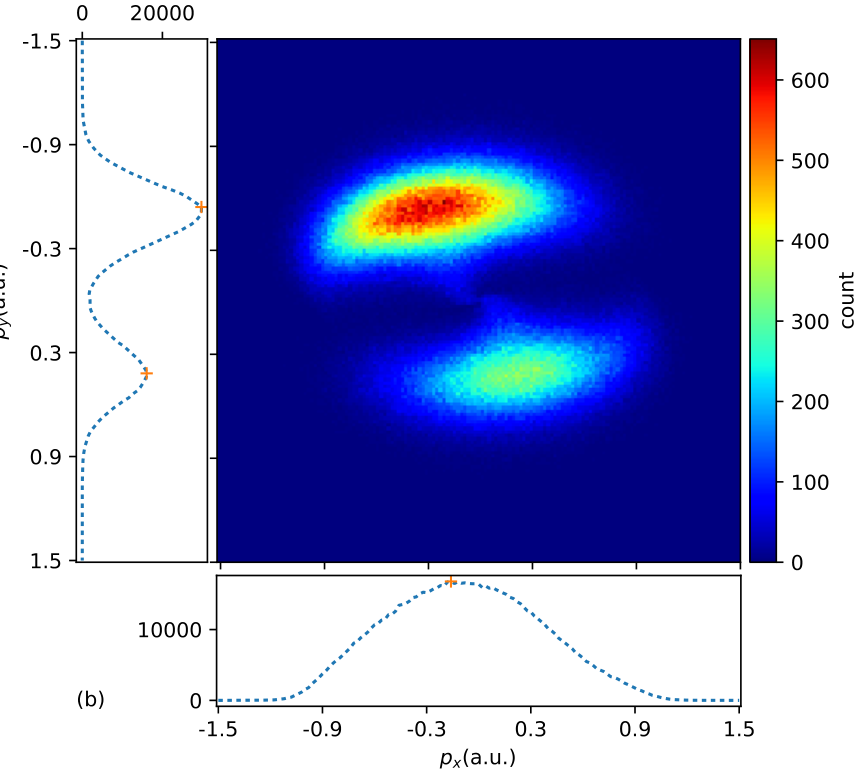
\includegraphics[width=10cm]{./fig/Prob2_4.png}
	\caption{椭圆偏振情况}
\end{figure}
对于线偏振的情况,$p_z$的先动量双峰谓语$-0.36$,$0.20\text{a.u.}$附近,而$p_y$的线动量分布单峰于$-0.02\text{a.u.}$附近。不难发现体系实际上对于$p_y$轴是对称的,这一点也可以在哈密顿量中反映出来。

对于椭圆偏振的情况,$p_z$的线动量分布单峰于$-0.16\text{a.u.}$附近,$p_y$线动量分布双峰于$-0.54$,$0.42\text{a.u.}$,同样出现了一强一弱两个区域。

这样的现象可以从电场强度的大小来分析。
\begin{figure}[hbt]
	\centering
	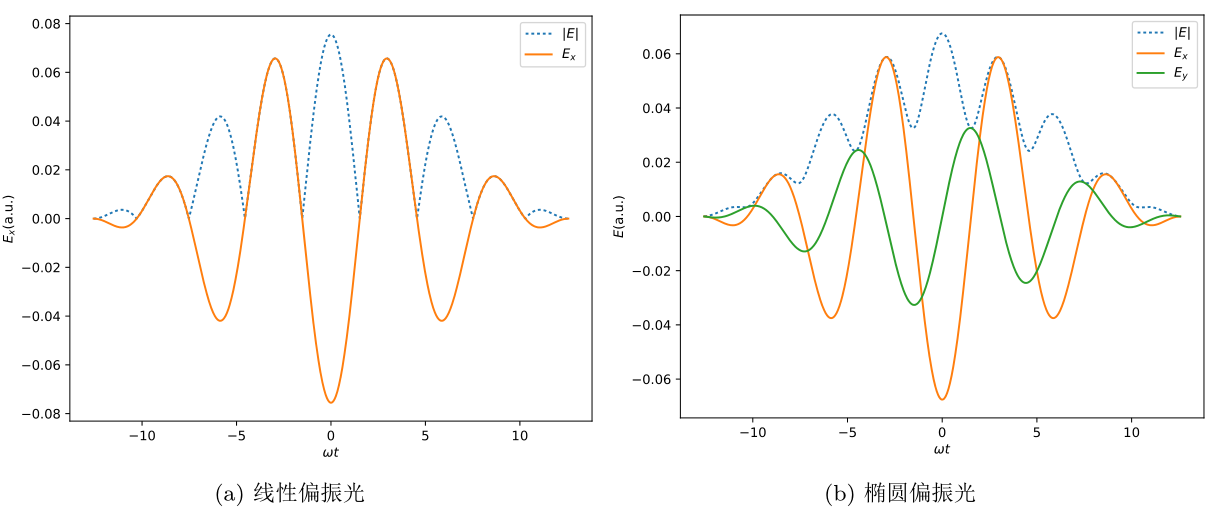
\includegraphics[width=8cm]{./fig/Prob2_2.png}
\end{figure}
由于电场强度越大,电离度越高,因此模拟结果出现的几个峰值应当是在电场最大的几个时刻所激发的电子。对于线偏振的情形,电子动量谱的两个峰是$t=0$和$t=3/\omega$时刻被激发电子所产生的。对于椭圆偏振,同样也是两个时刻激发的电子,只是因为电场的方向不同导致在动量空间有一个转动。但是二者整体性质还是类似的。
\section{第三题:FPU问题}
FPU模型是世界上第一个计算物理模型,它讨论的是一维弹簧振子链,两端点固定,体系哈密顿量:
\begin{equation}
H=\sum_{j=1}^{n} \frac{1}{2} p_{j}^{2}+\sum_{j=0}^{n} V\left(q_{j}-q_{j+1}\right)
\end{equation}
\begin{equation}
V(\Delta q)=\frac{1}{2}(\Delta q)^{2}+\frac{\alpha}{3}(\Delta q)^{3}+\frac{\beta}{4}(\Delta q)^{4}
\end{equation}
当$\alpha = \beta = 0$时,这就是经典的谐振子模型。
\subsection{谐振子守恒量}
引入简正坐标之后
\begin{equation}
Q_{k}=\sqrt{\frac{2}{n+1}} \sum_{j=1}^{n} q_{j} \sin \frac{\pi k j}{n+1}
\end{equation}
可以通过傅里叶变换得到将质点的坐标用简正坐标表示出
\begin{equation}
q_{j}=\sqrt{\frac{2}{n+1}} \sum_{k=1}^{n} Q_{k} \sin \frac{\pi k j}{n+1}
\end{equation}
\begin{equation}
p_{j}=\sqrt{\frac{2}{n+1}} \sum_{k=1}^{n} \dot{Q}_{k} \sin \frac{\pi k j}{n+1}
\end{equation}
将变换后的的动量和坐标代入哈密顿量可以得到:
\begin{equation}
H_{0}=\sum_{j=1}^{n} \frac{1}{2}\left(\dot{Q}_{k}^{2}+\omega_{k}^{2} Q_{k}^{2}\right), \quad \omega_{k}=2 \sin \frac{\pi k}{2(n+1)}
\end{equation}
这样系统有一系列脱耦的模式(声子),从而就有一系列守恒量:
\begin{equation}
E_{k}=\frac{1}{2}\left(\dot{Q}_{k}^{2}+\omega_{k}^{2} Q_{k}^{2}\right)
\end{equation}
在之后的代码实现之后,也可以证明各模式能量守恒
\begin{figure}[hbt]
	\centering
	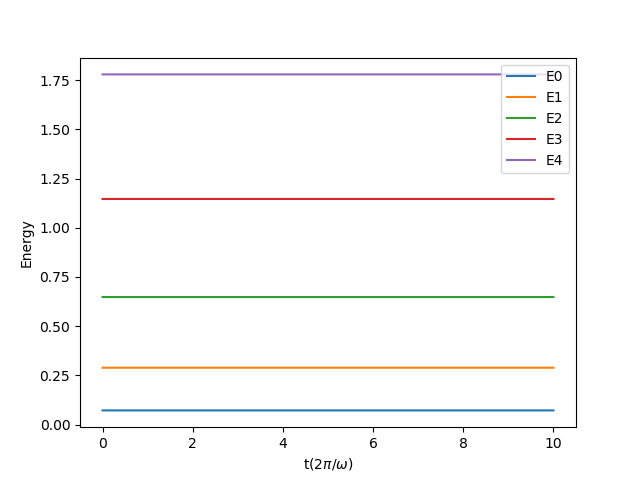
\includegraphics[width=8cm]{./fig/Prob3_1.png}
	\caption{守恒情况下的声子模}
\end{figure}
\subsection{核心代码}
\begin{lstlisting}
class phonon:
	dt = 0.1
	def __init__(self,Q0,Q00,a=0):
		self.alpha=a
		self.Q = Q0[:]
		self.Q_dot=Q00[:]
		self.__n = len(self.Q)
		self.__Trans_q()
		self.omega=2*np.sin(np.pi*0.5/(self.__n+1))
\end{lstlisting}
本题的大部分都在声子类方法完成。

声子的演化也上题中类似,采用RK-4算法完成。
\begin{lstlisting}
def __q_evolve(self,p):
	'''
	返回\ dot q
	'''
	return p[:]

def __p_evolve(self,q):
	'''
	返回\ dot p
	'''
	tq = [0]+q+[0]
	return\
	[tq[i-1]-2*tq[i]+tq[i+1]+self.alpha*((tq[i-1]-tq[i])**2-(tq[i]-tq[i+1])**2)\
for i in range(1, n+1)]

def Evolve(self):
	'''
	演化函数,只演化一步
	利用RK-4
	'''
	n = self.__n
	kq1 = self.__q_evolve(self.p)
	kp1 = self.__p_evolve(self.q)
	kq2 = self.__q_evolve([self.p[i]+.5*self.dt*kp1[i] for i in range(n)])
	kp2 = self.__p_evolve([self.q[i]+.5*self.dt*kq1[i] for i in range(n)])
	kq3 = self.__q_evolve([self.p[i]+.5*self.dt*kp2[i] for i in range(n)])
	kp3 = self.__p_evolve([self.q[i]+.5*self.dt*kq2[i] for i in range(n)])
	kq4 = self.__q_evolve([self.p[i]+self.dt*kp3[i] for i in range(n)])
	kp4 = self.__p_evolve([self.q[i]+self.dt*kq3[i] for i in range(n)])
	# 更新q,p
	self.p = [self.p[i]+self.dt/6*(kp1[i]+2*kp2[i]+2*kp3[i]+kp4[i])
	for i in range(n)]
	self.q = [self.q[i]+self.dt/6*(kq1[i]+2*kq2[i]+2*kq3[i]+kq4[i])
	for i in range(n)]
	# 更新Q,Q_dot
	self.__Tans_Q()
\end{lstlisting}
\subsection{短周期}
选取$\alpha  =0.25$和$Q_1(0)=4$,可以计算得到前五个模式随时间演化的关系
\begin{figure}[hbt]
	\centering
	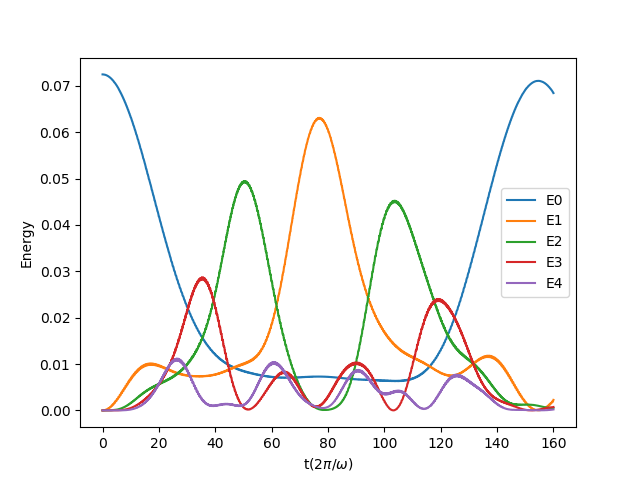
\includegraphics[width=10cm]{./fig/Prob3_2.png}
	\caption{短周期下系统前五个模式的演化}
\end{figure}
从图中可以读出大约在$t=156T$左右系统回到初态。

此时系统能量的分配可以做出图:
\begin{figure}[hbt]
	\centering
	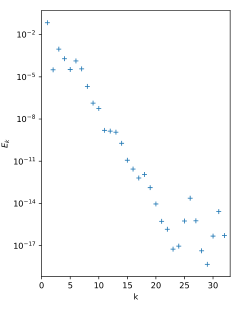
\includegraphics[width=8cm]{./fig/Prob3_4.png}
	\caption{各模式的能量分布}
\end{figure}
此时$E_1$占到所有模式总能量的$98\%$
\subsection{对回归的解释}
首先这一结果是反直觉的,但是可以有两个合理的解释:
\begin{enumerate}
	\item 第一种可能的解释是:FPU总的来说是一个振子模型,在激发足够小的时候,体系仍然可以视为一个谐振子模型加上微扰项。但是实际上会发现,高次相互作用并不是微扰,而不同能量间的耦合可以很大(例如$E_1$的能量可以接近于零)。因此这不太可能是这个问题的实质性原因。
	\item 第二种解释:注意到,当$E_1$下降时,主要激发的是与之相近的几个声子模式,从物理图像上理解,非线性项使得声子间产生耦合,在哈密顿量中引入了双声子、三声子相互作用,即$Q_{k} Q_{l} Q_{m}$这种作用项。在这些交叉项中,相近的模式会是主要贡献。因此可以猜测这种准周期运动的另一种可能是k空间的近局域耦合之后声子出现的一种拍频行为。
\end{enumerate}
\subsection{大尺度回归}
当将时间尺度放到$4000T$,会发现时间更长的回归周期。

\end{document}